\section{Validation without selections}
\label{sec:validation}

%This section validates the parameterization and the basis on the generated samples
%themselves, with no selection applied. The behaviour under a realistic selection is the
%subject of Sec.~\ref{sec:validation_realistic}.

The basis search returns the basis with the lowest score, exhibited in Table~\ref{tab:smeft_basis_9d}, which can be further validated using all the generated samples not selected as BPs. Here the BPs are used in the matrix method applied to LHE events in the absence of any selection. The bin-level quantities of Ref.~\cite{HH_nonggf_R5} are used to investigate the accuracy of the modeling provided by the matrix method using the proposed BPs: the relative residual $(N_\mathrm{interp}-N_\mathrm{MC})/N_\mathrm{MC}$, the relative propagated interpolation uncertainty $\sigma_\mathrm{interp}/N_\mathrm{MC}$ of Eq.~\eqref{eq:sigmainterp}, and the pull $(N_\mathrm{interp}-N_\mathrm{MC})/\sqrt{\sigma^2_\mathrm{interp}+\sigma^2_\mathrm{MC}}$. Furthermore, with the savings in MC production time (ELR, $A$-coefficients) and computing resources required for the full experimental analysis workflow over a 9D scan (MM), the combination of both methods provides a crucial scheme for accessing the rich theory space of EFTs such as SMEFT, and is therefore explored in the upcoming sections. For the following tests, the shapes obtained solely from the $A$-coefficients serve as a reference baseline for the accuracy achieved with by the MM and MM+ELR approaches.

%but the score is a ranking
%device and not a statement about accuracy, and how well it stands in for one depends on
%the parameterization: over the seeds of a sweep its rank correlation with the held-out
%median shape error is $+0.61$ for the nominal nine-coefficient basis and $+0.07$ for the
%fifteen-point one, where it instead tracks the tail of the residual distribution. A
%finished basis is therefore validated separately from being selected. The validation
%uses the samples that are not themselves basis points --- $4336$ of them for the nominal
%parameterization --- so that nothing is scored on its own input, 

%with the bin-level quantities of Ref.~\cite{HH_nonggf_R5}: the relative residual $(N_\mathrm{interp}-N_\mathrm{MC})/N_\mathrm{MC}$, the relative propagated interpolation uncertainty $\sigma_\mathrm{interp}/N_\mathrm{MC}$ of Eq.~\eqref{eq:sigmainterp}, and the pull $(N_\mathrm{interp}-N_\mathrm{MC})/\sqrt{\sigma^2_\mathrm{interp}+\sigma^2_\mathrm{MC}}$.

\subsection{Kinematic behaviour of the basis points}
\label{sec:validation_shapes}
\label{sec:validation_nsamples}

The basis has forty points and can be sorted into four kinematic regimes. The number of regimes are separated according to the behavior of the shape at the interference regions $2m_{\text{H}}$ (threshold), $2m_{\text{t}}$, and in the high-mass tail. Normalizing each point to its own yield and grouping by the shape of the \mHH distribution, Fig.~\ref{fig:basis_shapes}, the same six structures highlighted in Ref.~\cite{Bär:2965348} are found. Such structures are given according to the rich diversity arisen from the interferences around the production threshold ($2m_\text{H}$) and $2m_t$, and also in terms of the similarity in relation to the SM shape. All the BPs found can be related to one of the six benchmarks defined in Ref.~\cite{Bär:2965348}.

%\footnote{Ref.~\cite{Bär:2965348} adds a new region where the contribution at $2m_{\text{H}}$ is not as suppressed as in the SM case. Here such samples are absorbed in what is quoted as "threshold-like". Furthermore, the "two peaks" region is also subdivided according to which peak ($2m_{\text{H}}$ or $2m_{\text{t}}$) is the dominant one.}. %It is well known that truncation effects can produce negative predictions in regions more sensitive to destructive interference between diagrams, and this can be seen in a small number of bins in Fig.~\ref{fig:basis_shapes}. Such effects are even more pronounced when restricted to the linear truncation, as just the SM-Dim6 interference is taken into account. Although unphysical, this is not a problem from the perspective of the modeling, are genuinely present in the kinematic space covered by the theory 

%. ...These come
%from the negative event weights of the next-to-leading-order generation where a sample has few events, they affect $0.5\%$ of bins, and they are not a truncation of the EFT expansion.

In a realistic scenario, the matrix method is often used together with the ELR: some of the BPs are directly produced with MC and then reweighted in a combined way to the remaining templates using bin-by-bin inverse-variance weights, namely the multi-ref approach discussed in Ref.~\cite{ELR_R5}. The identification of the shape properties helps to answer the question regarding which BPs must be chosen to be generated. The left panel in Figure~\ref{fig:elr_sources} shows the median relative shape residual as a function of the number of input points used in the ELR of all the remaining BPs required by the MM approach. Reference lines are drawn for the results obtained directly with the $A$-coefficients, and by the MM using all BPs directly generated by MC. The median is computed by comparing the shapes given by all three modeling techniques with all the generated samples (\ref{tab:grids_comp}), except for the BPs. The higher value given by the MM with 40 generated points is expected, as it carries the statistical fluctuations of each of the forty samples, something that is absent in the $A$-coefficients. By using the MM with points obtained through the multi-ref approach in an increasing number of BPs, the median drops towards the optimal value given by the $A$-coefficients, but saturates around six source samples, meaning that one BP representing each of the six kinematic groups sets an stable point to the MM+ELR approach. The particular combination of samples used in each of the blue markers starts first with the SM, since its the sample that any analysis generates anyway, and then proceeds by incrementally including any sample of the remaining five kinematic regimes once all of them are represented at least once. The right panel shows the shapes of the selected BPs used in the MM+ELR approach in the six-source point of the left panel. As expected, the effect of changing different BPs inside a given kinematic group it was found to be small. The distributions of the relative shape residual corresponding to the medians shown in Figure \ref{fig:elr_sources} are exhibited in Figure \ref{fig:closure_9d}, for the $A$-coefficients evaluated directly (blue), MM (orange), and MM+ELR (six sources, green).





%The matrix method can be used
%It is the number of regimes rather than the number
%of points that sets how many samples have to be simulated, which is what the rest of this
%subsection establishes.

%The regimes are separated by how much yield they place at high mass. Of each sample's
%yield, the fraction above $1$~TeV is $5.3\mbox{--}19.7\%$ for the hard-tail points,
%$0.0\mbox{--}7.2\%$ for the two-peak points, $0.0\mbox{--}4.9\%$ for the threshold-like
%points and $0.8\mbox{--}3.6\%$ for the SM-like ones, the SM itself at $0.8\%$. Above
%$1.2$~TeV the ordering holds with $3.2\mbox{--}13.7\%$, $0.0\mbox{--}3.3\%$,
%$0.0\mbox{--}2.4\%$ and $0.2\mbox{--}1.5\%$. A hard-tail point puts an order of magnitude
%more of its events where the spectrum is least populated than an SM-like one, so a set of
%samples covering the regimes constrains the tail better than one covering the coupling
%space uniformly.


\begin{figure}[htbp]
    \centering
    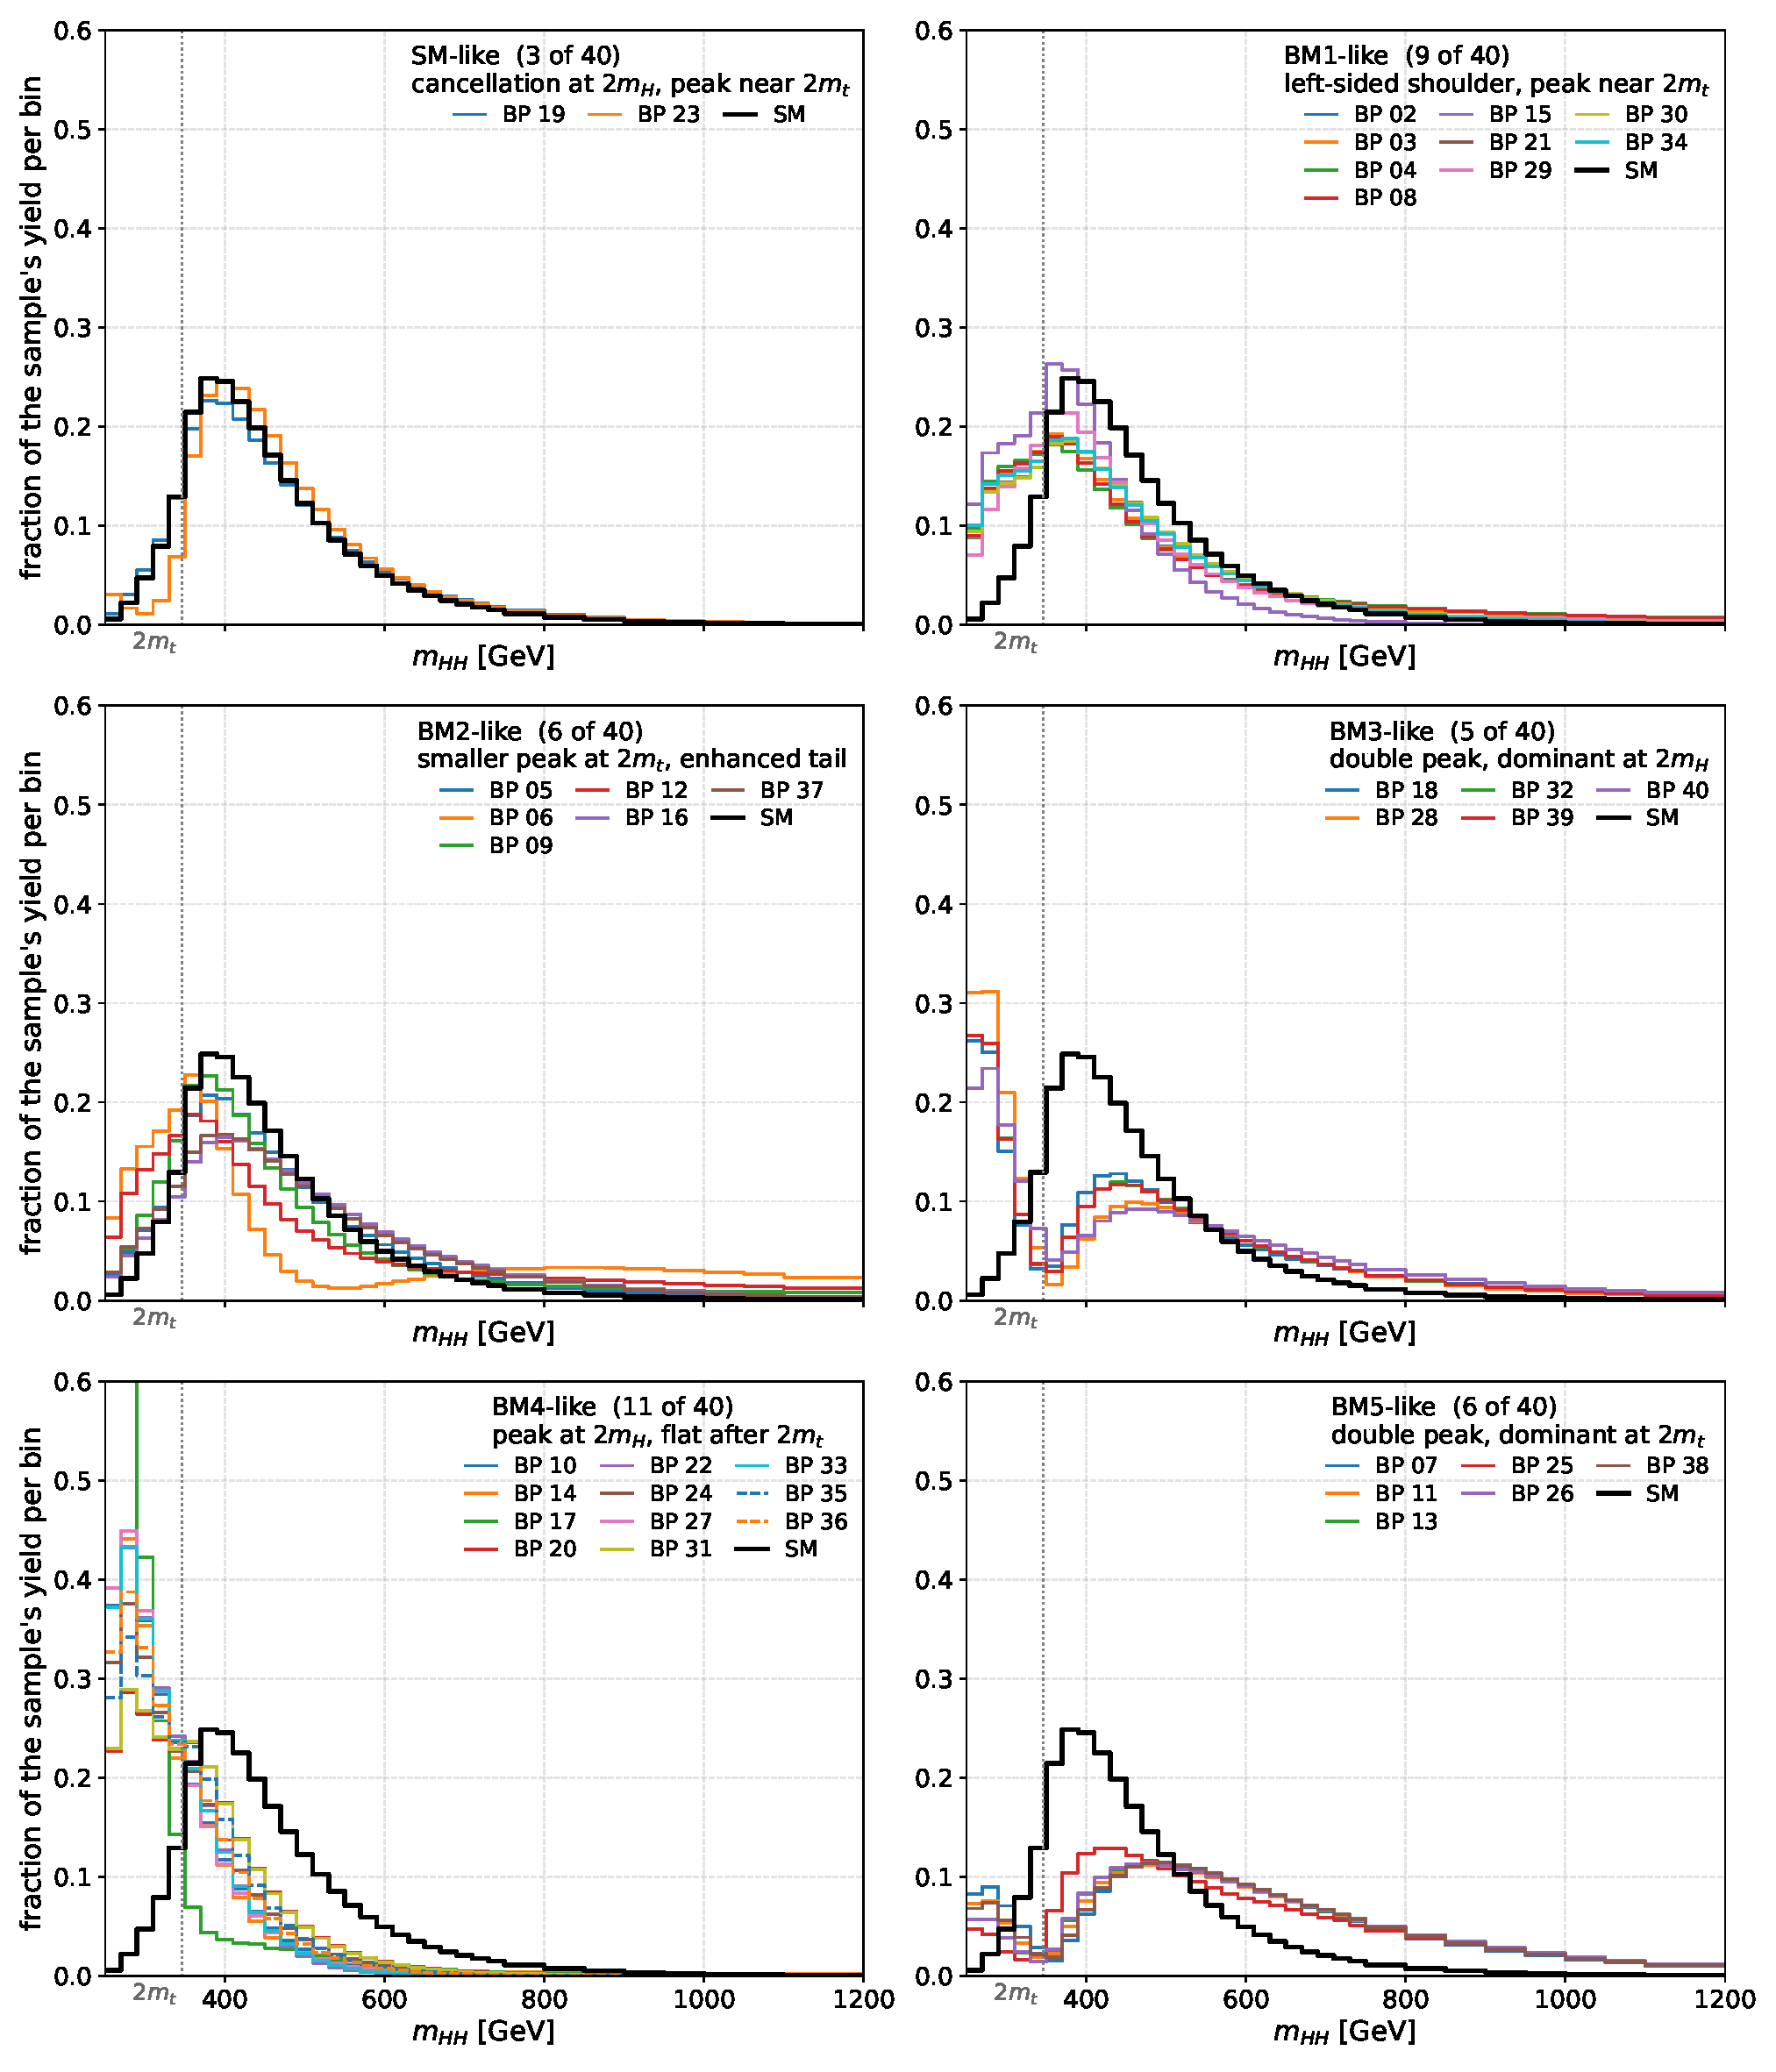
\includegraphics[width=1.025\textwidth]
        {plots/mHH_shape_classes_6panel_BMfeatures_newbasis_1.pdf}
    \caption{Normalized \mHH distribution of each of the forty basis points, grouped under each of the six identified shape features, with the SM drawn in black in every panel.}
\label{fig:basis_shapes}
\end{figure}
\begin{figure}[htbp]
    \centering
    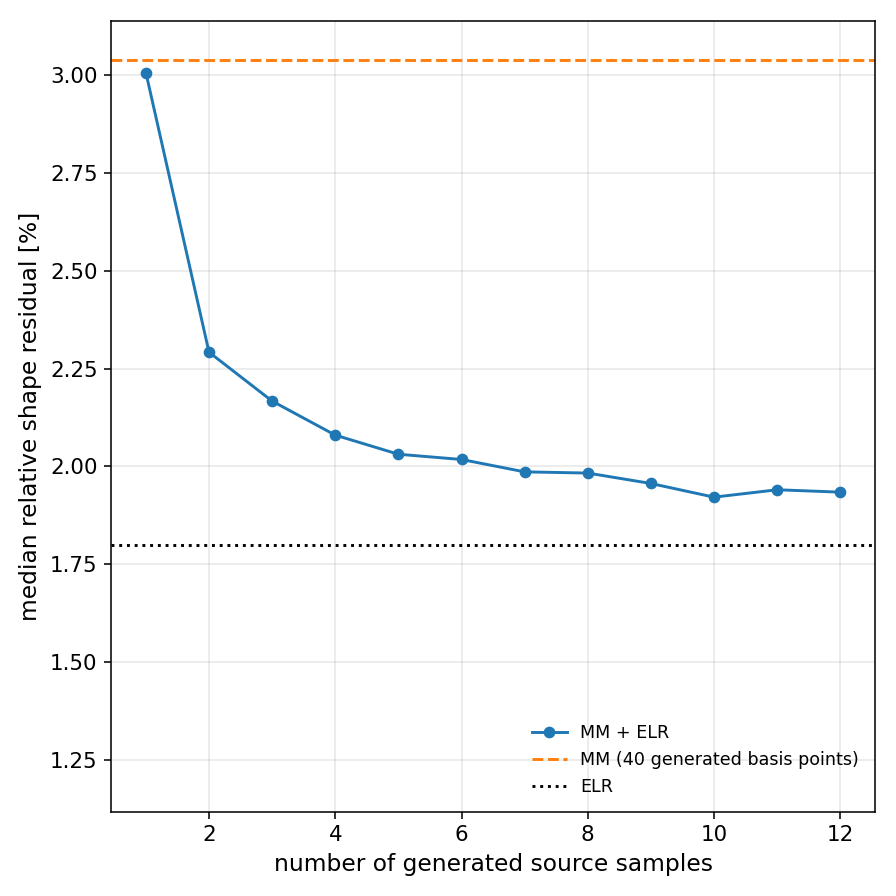
\includegraphics[width=0.47\textwidth]
        {figures/basis_optimization/elr_source_scan.png}
    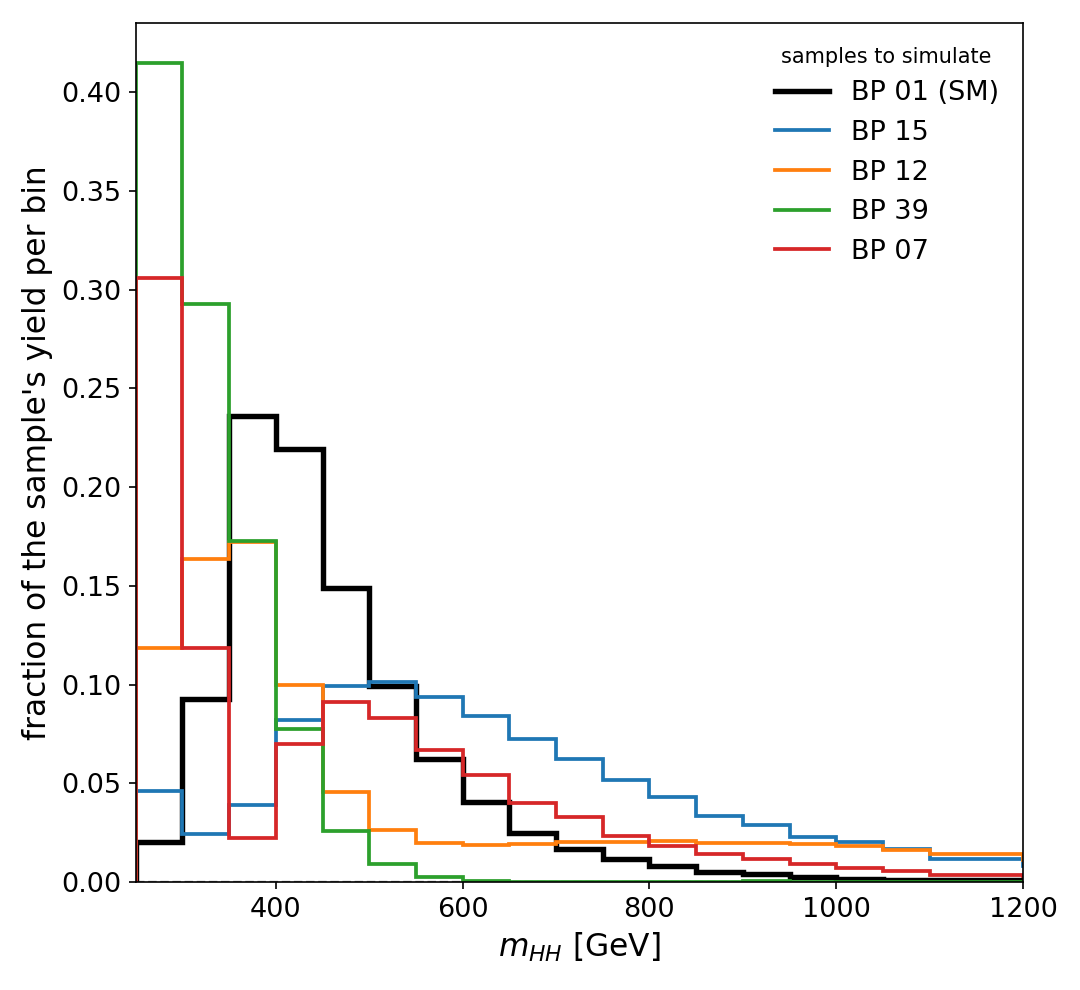
\includegraphics[width=0.51\textwidth]
        {figures/basis_optimization/elr_sources_5_mHH.png}
    \caption{Left: median relative shape residual of the forty-point basis when
    its templates are built by reweighting from a given number of generated
    source samples and combined per bin with inverse-variance weights, against
    the basis taken entirely from generated samples (dashed) and the distributions
    evaluated directly from the $A$-coefficients (dotted). Right: the \mHH distributions of the five
    samples used for the five-source point of the left panel, each normalized to its own yield.}
    \label{fig:elr_sources}
\end{figure}


%The residual of the matrix method is dominated by the statistics of its basis samples, so
%it is reduced by making those templates more precise. The price of doing that by
%simulation can be read off. Taking the reweighting fit evaluated at each basis point as a
%noise-free template and adding Gaussian noise of the size the real samples carry
%reproduces the delivered closure to about $15\%$ --- $3.5\%$ against the $3.0\%$
%observed --- and scaling that noise by $1/\sqrt{f}$ gives what $f$ times the events would
%deliver: $2.4\%$ at $f=5$, $2.2\%$ at $f=10$ and $2.0\%$ at $f=20$.

%The same precision is obtained instead by \emph{building} each basis template from a few
%simulated samples by reweighting, combined bin by bin with inverse-variance weights as in
%Ref.~\cite{ELR_R5}. The residual falls from $3.0\%$ with one source to $2.03\%$ with
%five, against $3.04\%$ with all forty simulated and a floor of $1.80\%$. Beyond five the
%improvement continues slowly --- $1.92\%$ at ten --- so the number to simulate is set by
%where the returns fall below the cost of a sample rather than by a plateau. The five
%sources are themselves basis points, so none of this asks for simulation outside
%Table~\ref{tab:smeft_basis_9d}. The left panel of Fig.~\ref{fig:elr_sources} shows the
%scan, approaching but not reaching the reweighting's own floor and lying below the
%$3.0\%$ of the basis as generated.

%Which samples are chosen is a smaller effect than how many, and it is set by the
%kinematics rather than by the coupling values. The five sources are drawn from the basis
%points, classified into the four regimes above. The SM is taken first, as the point
%every analysis simulates in any case; the remaining four are taken one regime at a time,
%and within a regime the point taken is the one furthest in normalized \mHH shape from
%everything already chosen, among those whose own statistics are no worse than half the
%median of the sample set. The order in which the regimes are visited is the one free
%choice, and weighting them equally is not the best rule: the hard tail is visited twice
%before the others are exhausted, because that is where the residual and its propagated
%uncertainty are largest, both growing by a factor $6\mbox{--}7$ between threshold and
%$2$~TeV, so a second sample there reduces the residual more than a second anywhere else.
%The gain is $2.03\%$ against $2.07\%$ at five sources --- five samples chosen this way
%reach what six reach when the regimes are weighted equally --- and it is specific to
%five, since at four sources every ordering tested gives $2.08\%$. The five that result
%span the spectrum rather than the coupling space: one peaks at threshold and is exhausted
%by $700$~GeV, two carry hard tails with yield beyond $1.2$~TeV, and the SM and one
%two-peak point fill the region between, so every bin of a reweighted template is
%%dominated by a source that has events in it, which is what the inverse-variance
%combination needs in order to improve on an average of noise. Selecting instead by
%distance from the SM in coupling space is worse at every number of sources, and erratic
%at small ones: its second pick makes the residual worse than one source alone, because it
%takes an extreme point with poor statistics.



%The two methods contribute different things. The reweighting supplies the precision: it
%carries the information of the full sample grid into every basis template, so a template
%is as precise as the fit rather than as precise as the one sample behind it. The matrix
%method supplies the form: an analytic function of the nine Wilson coefficients, built
%once, through which a likelihood scan moves continuously, which a reweighting evaluated
%point by point does not provide. Used together, the forty templates of
%Table~\ref{tab:smeft_basis_9d} need five fully simulated samples behind them.

%Choosing the basis well is itself a saving in simulation, and the same noise model prices
%it. An earlier basis, found by the same search but allowed two points outside the
%two-dimensional planes, closed at $3.54\%$ against the $3.04\%$ of the basis adopted
%here. Reaching the latter with the former would have taken about twice the events in
%every one of its forty samples, and reaching the level that reweighted templates deliver
%would have taken fifty times rather than twenty. A basis is therefore not only a choice
%of where to evaluate the parameterization but a choice of how much simulation the result
%will cost, and the two are optimized together.

%Stated as an analysis would see it: the reweighting coefficients are an input, extracted
%once from the grid of Sec.~\ref{sec:grids} and provided with this report, not something a
%user re-derives. Reaching the $2.03\%$ that five reweighted samples deliver by generating
%instead would take about twenty times the events in each of the forty basis samples,
%equivalent to some eight hundred samples against five. The gain is in cost rather than in
%accuracy: $3.04\%$ to $2.03\%$ is a third off the residual, and the two matrix-method
%curves of Fig.~\ref{fig:per_bin} lie on top of each other. Three things follow for an
%analysis. The templates are more precise, so the interpolation adds little to the
%statistical error of the result; the simulation request is five samples rather than
%forty; and the bookkeeping an analyzer carries --- samples to request, track, calibrate
%and systematically vary --- is reduced in the same proportion.
\begin{figure}[t]
    \centering
    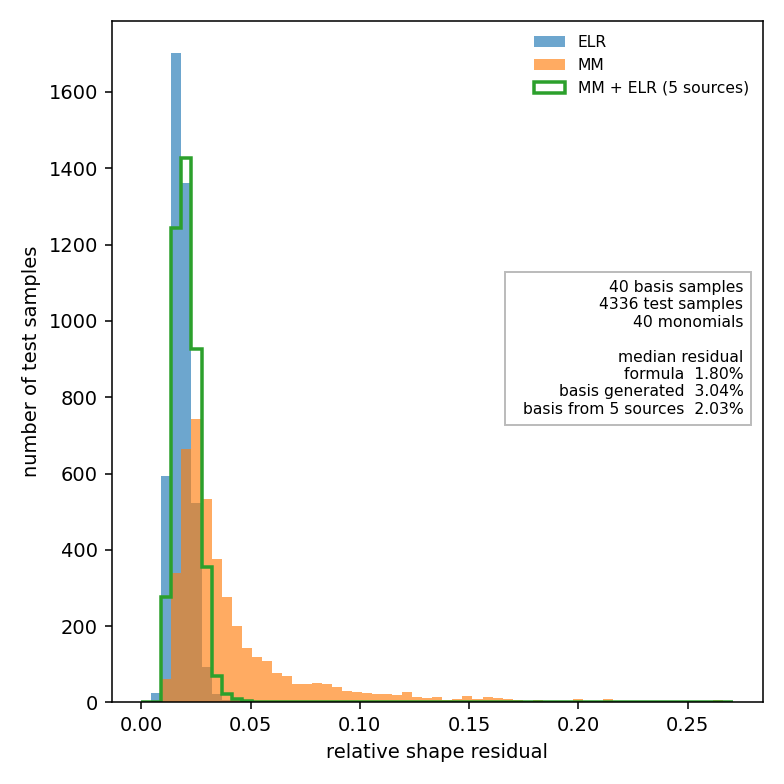
\includegraphics[width=0.48\textwidth]
        {figures/basis_optimization/closure_decomposition_9d.png}
    \caption{Distribution of the relative shape residual, medians quoted in the panel. The distributions correspond to the same median values shown in Figure \ref{fig:basis_shapes}.}
\label{fig:closure_9d}
\end{figure}


\subsection{Closure of the matrix method}
\label{sec:validation_mm}

\begin{figure}[htbp]
    \centering
    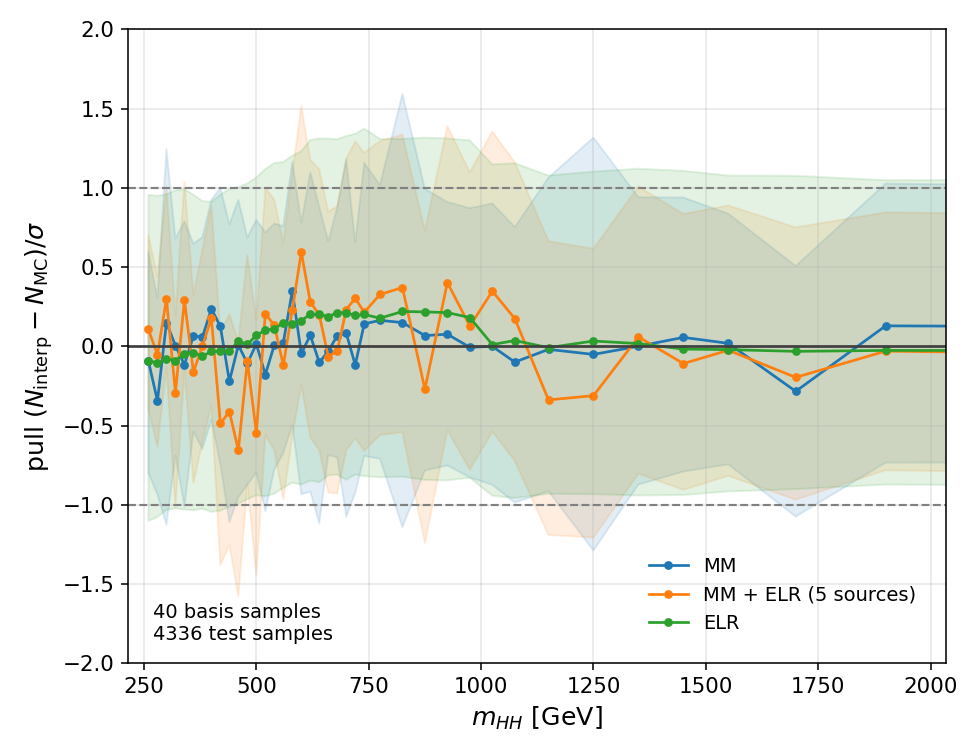
\includegraphics[width=0.62\textwidth]
        {figures/basis_optimization/per_bin_pull_9d.png}
    \caption{Pull per \mHH bin,
    $(N_\mathrm{interp}-N_\mathrm{MC})/\sqrt{\sigma^2_\mathrm{method}+\sigma^2_\mathrm{stat}}$,
    for the matrix method on the basis as generated (MM), with its templates
    built by reweighting from the six sources (MM+ELR), and for the
    $A$-coefficients evaluated directly. Points are the median over the $4336$
    samples and bands the central $68\%$ confidence level. An unbiased prediction has its
    median on zero. A correctly estimated uncertainty gives a band reaching
    $\pm1$, marked by the dashed lines.}
    \label{fig:per_bin}
\end{figure}
\begin{figure}[htbp]
    \centering
    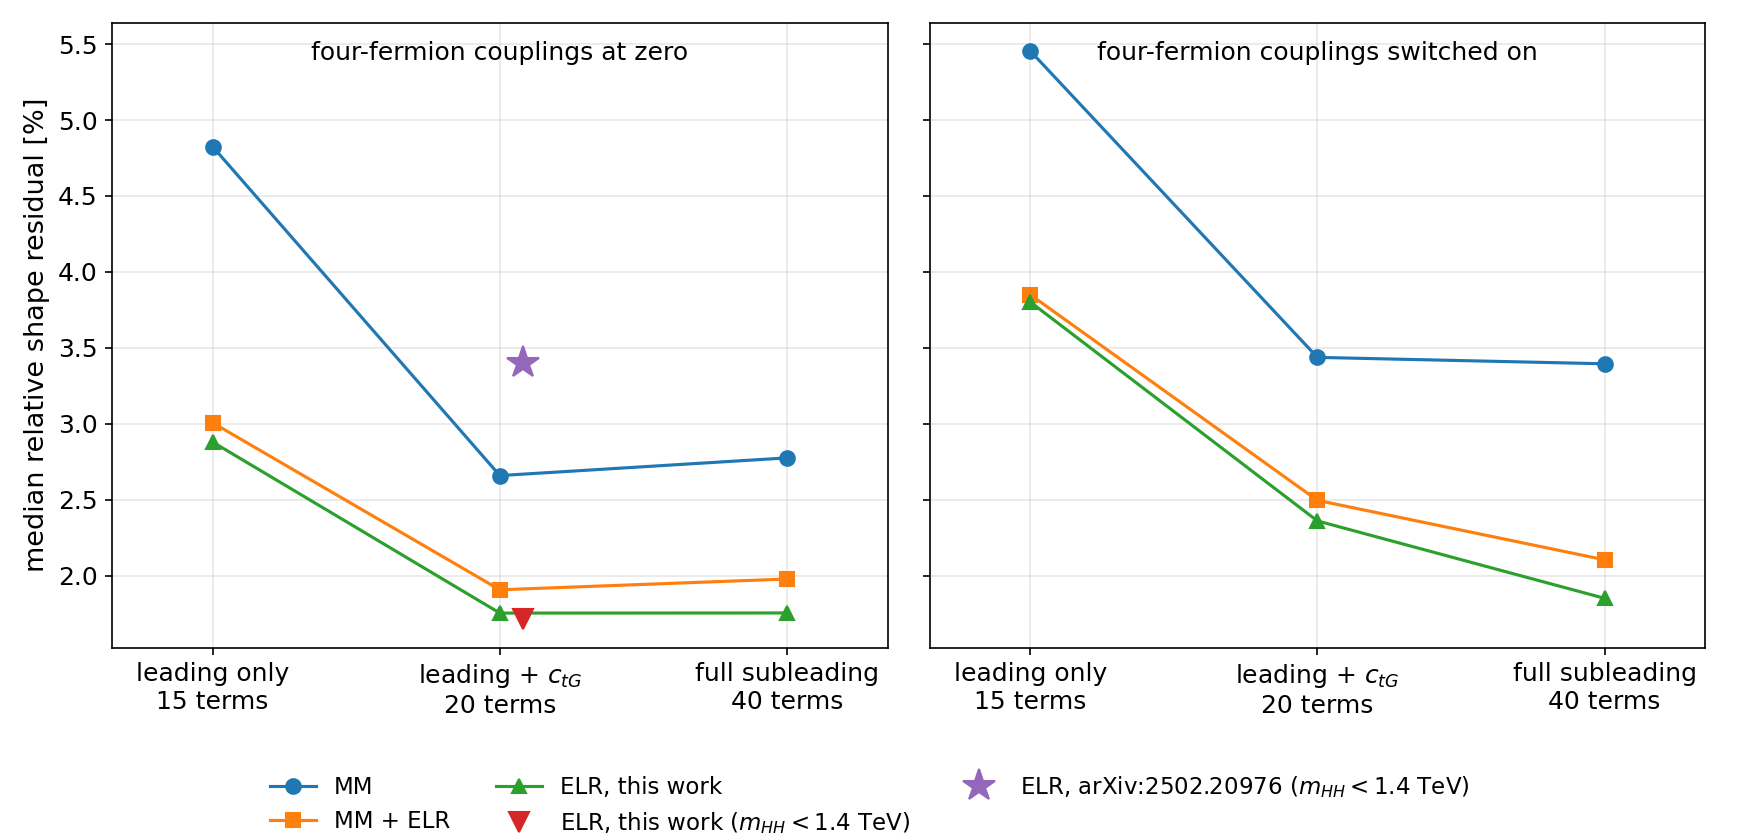
\includegraphics[width=0.96\textwidth]
    {figures/basis_optimization/ladder_comparison.png}
    \caption{Median relative shape residual against the generated samples for three
parameterizations of increasing operators coverage, evaluated on the same $4376$ samples. The panels
separate the samples with the four-fermion coefficients at zero (left) from those with at
least one switched on (right). In the latter case, the leading-only and leading+$c_{tG}$ parameterizations neglect the effects of the four-fermion operators as they are by construction insensitive to them.}
\label{fig:ladder}
\end{figure}

In order to further assess the accuracy found with the recommended BPs, one can look at the pull distributions and investigate how close they are from a Gaussian-like behavior. It can be noticed from Figure \ref{fig:per_bin} that all the distributions fluctuates around zero for the whole $m_\HH$ spectrum. Each point corresponds to the median value over all samples, except for the BPs. All distributions sits well within the $\pm1\sigma$ bands, showing reasonable agreement with an unbiased modeling. 

Additionally, we investigate the results obtained with BPs found for different operators coverage, as described in Figure \ref{fig:ladder}. In particular, for the case restricted to the leading plus chromomagnetic operators, the results can be compared to the ones found with other $A$-coefficients available in the literature \cite{Cadamuro:2025car}\footnote{The coefficients derived in this reference goes only up to $m_\HH=1.4$ TeV. Therefore, for a fair comparison,  the red marker in Figure \ref{fig:ladder} is given by our coefficients evaluated on the same range.} that cover the same set of operators. Given the observed values for the median relative shape residual, a systematic improvement can be observed in all cases (MM, MM+ELR and the $A$-coefficients of this work). Leading-only and leading+$c_{tG}$ parameterizations neglect the additional terms related to the four-fermion operators, and the effect of this is an increase of $\sim1\%$ in the shape residual in the right-side panel regarding the entries for 15 and 20 terms, meaning that in general the four-fermion operators produce very subtle changes in the shapes.

ADD FINAL COMMENTS ABOUT OTHER BASES AND THE FINAL RECOMMENDED ONE.

%The optimized bases reproduce their own parameterization exactly: interpolating the
%$A$-coefficients themselves rather than the simulated yields returns them to a relative
%$10^{-15}$. The residual against the simulated samples is therefore not interpolation
%error. It has two contributions, which can be separated because the reweighting of
%Sec.~\ref{sec:extraction} describes the same cross section independently: the accuracy of
%the parameterization itself, and the Monte Carlo statistics of the basis samples
%amplified by the interpolation weights. For the nominal basis the first is $1.8\%$ and
%the total $3.0\%$ in median relative shape residual, so most of what the matrix method
%adds is the statistical error of its forty samples rather than a failure to describe the
%physics. The pull is close to a standard normal and slightly narrower --- $74.7\%$ of
%entries within $1\sigma$ and $97.1\%$ within $2\sigma$, against $68.3\%$ and $95.4\%$ ---
%so the quoted interpolation uncertainty covers the observed scatter and is conservative
%by about a quarter.

%The left panel of Fig.~\ref{fig:closure_9d} shows the distribution of the residual over
%the test samples for the three cases. What separates the medians of the reweighting and
%the matrix method is not a shift of one narrow distribution relative to another: the
%cores largely overlap, and the difference is a tail of test samples extending beyond
%$10\%$ where the reweighting stops below $5\%$. That is the signature of a statistical
%effect concentrated on the samples whose prediction leans on the least populated
%templates. Building the basis templates by reweighting from five sources removes the tail
%and returns the median to $2.03\%$, against $1.80\%$ for the reweighting itself and
%$3.04\%$ for the basis as generated.

%One alternative explanation can be excluded directly. If the excess came from a minority
%of test points that the interpolation reaches only through large, cancelling weights, it
%would track the size of those weights. It does not: correlating the residual with
%$\sum_i|w_i|$ over the test set gives $-0.10$ for the matrix method, and the comparison
%with the reweighting is unchanged at every weight norm, the right panel of
%Fig.~\ref{fig:closure_9d}. The excess is a property of the precision of the forty
%templates as a set, which is why improving those templates removes it everywhere rather
%than only in the badly conditioned corners.

%\begin{figure}[htbp]
%    \centering
%    \includegraphics[width=0.48\textwidth]
%        {figures/basis_optimization/closure_decomposition_9d.png}
%    \includegraphics[width=0.48\textwidth]
%        {figures/basis_optimization/residual_vs_weight_9d.png}
%    \caption{Closure of the nominal nine-coefficient basis over the $4336$ generated samples
%that are not themselves basis points, for the reweighting fit evaluated directly (ELR),
%the matrix method on the basis as generated (MM), and the matrix method with every basis
%template built by reweighting from five generated samples (MM\,+\,ELR). Left:
%distribution of the relative shape residual, medians quoted in the panel. Right: the same
%residual against the summed magnitude of the interpolation weights, with the correlation
%quoted in the panel.}
%\label{fig:closure_9d}
%\end{figure}

\label{sec:validation_perbin}
%Those quantities are medians over the whole \mHH range. Resolved bin by bin the relative
%residual rises by a factor $6.1$ between the threshold region and $2$~TeV for the matrix
%method. Dividing by the uncertainty that should account for it, Fig.~\ref{fig:per_bin}
%shows the pull $(N_\mathrm{interp}-N_\mathrm{MC})/\sigma$ with
%$\sigma^2=\sigma^2_\mathrm{method}+\sigma^2_\mathrm{stat}$, combining the statistical
%error of the test sample with the propagated uncertainty of the prediction. Those differ
%between the three: the matrix method on generated templates carries the statistics of its
%forty basis samples, the same method on reweighted templates the smaller uncertainty of
%an inverse-variance combination, and the reweighting evaluated directly neither.

%The median tests for bias and sits at zero for all three across the spectrum, $+0.01$,
%$+0.03$ and $+0.03$ overall. The width tests the uncertainty, and the $68\%$ bands span
%$[-0.81,+0.87]$, $[-0.75,+0.89]$ and $[-0.93,+1.11]$ against the $\pm1$ of a correctly
%estimated error: the reweighting is calibrated and the two matrix-method cases are
%slightly narrow. The rise of the unnormalized residual with \mHH is accounted for by the
%growth of these two statistical errors, the test samples having three orders of magnitude
%less yield in the last bin than in the first.

%The bin-to-bin wander of the median is larger for the reweighted templates than for the
%generated ones, $0.28$ against $0.13$. The quantities behind the two numbers set that in
%context. The reweighted case has the smaller absolute residual, $2.03\%$ against
%$3.04\%$, and its worst test sample closes at $5\%$ where the generated basis reaches
%$70\%$. What the pull divides by is smaller still: the uncertainty of an inverse-variance
%combination is $0.55$ times the statistical error of a test sample, where the generated
%basis gives $1.51$, so the same deviation in cross section is displayed about three times
%larger. One contribution to the extra wander is that the five sources are reweighted with
%the same fitted coefficients and so are not strictly independent, which the
%inverse-variance combination assumes; the per-bin weighting removes most of that.


%The medians conceal a difference between the methods. The distribution of the residual
%over the test samples has a long tail for the matrix method on generated templates and
%a short one for the other two: the $99$th percentile is $23.8\%$ and the worst
%single sample reaches $70\%$, against maxima of $5.1\%$ and $5.2\%$ for the reweighted
%templates and the reweighting itself. The tail is not an artefact of a few pathological
%samples --- removing the worst $5\%$ moves the median only from $3.04\%$ to $2.95\%$.

%The $70$ samples with a residual above $20\%$, $1.6\%$ of the test set, have a median
%cross section of $23$~fb against $240$~fb for the test set as a whole, and the rank
%correlation between cross section and residual is $-0.74$. These are the points where the
%contributions cancel and the rate is small, so a given absolute error is a large relative
%one; the diagonal ridge of Fig.~\ref{fig:closure_9d} is the same feature seen in a
%coupling plane. The pull does not show a tail there, so the interpolation uncertainty
%already covers it. Building the basis templates by reweighting removes the tail: the
%median goes from $3.04\%$ to $2.03\%$ and the worst case from $70\%$ to $5\%$.

%\subsection{Effect of increasing dimensionality on the fit}
%\label{sec:validation_ladder}

%Adding coefficients to the parameterization adds terms to be solved for and samples to be
%simulated. Scoring every parameterization on the same samples --- the full
%nine-coefficient set, rather than each on the region where it happens to be exact ---
%measures what each step up buys. With the four-fermion coefficients at zero the
%twenty-term parameterization is already exact and the forty-term one adds nothing, both
%at $1.8\%$: the extra twenty terms describe operators that are switched off. With the
%four-fermion coefficients switched on the forty-term parameterization is the only one
%that keeps improving, $1.9\%$ against $2.4\%$. The gain is the recovery of a sector the
%smaller parameterizations cannot represent at all, which is the behaviour found for the
%ladder of Ref.~\cite{HH_nonggf_R5}.

%The published coefficients of Ref.~\cite{ELR_topdipole} are compared only where they are
%defined. Their fit stops at $m_{HH}=1.4$~TeV, so both they and our own twenty-term
%coefficients are evaluated on exactly the bins below it, and neither is favoured by the
%range. Extending them naively over the full range instead --- holding the last fitted bin
%constant in density, which is what an analysis using that formula at high mass would be
%forced to assume --- gives $13.15\%$ against the $3.40\%$ obtained where the fit is
%defined, with five of the forty bins extrapolated. That number measures the extrapolation
%and not the fit, which is why it is quoted here rather than drawn.

%Fig.~\ref{fig:ladder} shows three curves. The reweighting curve is the parameterization
%alone and improves monotonically along the ladder, $3.80$, $2.36$, $1.85\%$ with the
%four-fermion coefficients switched on. The matrix-method curve adds the statistical error
%of the basis samples, which is why it improves much less over the last rung, $3.44$ to
%$3.40\%$: forty basis samples carry more statistical error than twenty, and that almost
%exactly cancels the gain from the richer description. Building the basis templates by
%reweighting separates the two effects and recovers it, $2.50$ to $2.11\%$. The ordering
%of the underlying parameterizations is therefore visible only once the basis statistics
%are removed. The cost of the extra dimensionality is paid in sample statistics rather
%than in the description, and it is a cost the reweighting removes.

%All three are evaluated on the same $4376$ samples, so a parameterization that omits
%operators pays for it here rather than being scored only where it is exact. The
%improvement with the size of the parameterization is confined to the right panel: with
%the four-fermion coefficients at zero, the twenty-term description is already exact.
